% Slides for talk on hydrogen fuel cells
% given in the department on October 27, 2003.
% 
% The original slides were in Prosper.  This file contains the
% translation of the original slides to Beamer.
% 
% Rouben Rostamian <rostamian@umbc.edu>
% August 31, 2004

\documentclass[10pt]{beamer}\usepackage[]{graphicx}\usepackage[]{xcolor}
% maxwidth is the original width if it is less than linewidth
% otherwise use linewidth (to make sure the graphics do not exceed the margin)
\makeatletter
\def\maxwidth{ %
  \ifdim\Gin@nat@width>\linewidth
    \linewidth
  \else
    \Gin@nat@width
  \fi
}
\makeatother

\definecolor{fgcolor}{rgb}{0.345, 0.345, 0.345}
\newcommand{\hlnum}[1]{\textcolor[rgb]{0.686,0.059,0.569}{#1}}%
\newcommand{\hlstr}[1]{\textcolor[rgb]{0.192,0.494,0.8}{#1}}%
\newcommand{\hlcom}[1]{\textcolor[rgb]{0.678,0.584,0.686}{\textit{#1}}}%
\newcommand{\hlopt}[1]{\textcolor[rgb]{0,0,0}{#1}}%
\newcommand{\hlstd}[1]{\textcolor[rgb]{0.345,0.345,0.345}{#1}}%
\newcommand{\hlkwa}[1]{\textcolor[rgb]{0.161,0.373,0.58}{\textbf{#1}}}%
\newcommand{\hlkwb}[1]{\textcolor[rgb]{0.69,0.353,0.396}{#1}}%
\newcommand{\hlkwc}[1]{\textcolor[rgb]{0.333,0.667,0.333}{#1}}%
\newcommand{\hlkwd}[1]{\textcolor[rgb]{0.737,0.353,0.396}{\textbf{#1}}}%
\let\hlipl\hlkwb

\usepackage{framed}
\makeatletter
\newenvironment{kframe}{%
 \def\at@end@of@kframe{}%
 \ifinner\ifhmode%
  \def\at@end@of@kframe{\end{minipage}}%
  \begin{minipage}{\columnwidth}%
 \fi\fi%
 \def\FrameCommand##1{\hskip\@totalleftmargin \hskip-\fboxsep
 \colorbox{shadecolor}{##1}\hskip-\fboxsep
     % There is no \\@totalrightmargin, so:
     \hskip-\linewidth \hskip-\@totalleftmargin \hskip\columnwidth}%
 \MakeFramed {\advance\hsize-\width
   \@totalleftmargin\z@ \linewidth\hsize
   \@setminipage}}%
 {\par\unskip\endMakeFramed%
 \at@end@of@kframe}
\makeatother

\definecolor{shadecolor}{rgb}{.97, .97, .97}
\definecolor{messagecolor}{rgb}{0, 0, 0}
\definecolor{warningcolor}{rgb}{1, 0, 1}
\definecolor{errorcolor}{rgb}{1, 0, 0}
\newenvironment{knitrout}{}{} % an empty environment to be redefined in TeX

\usepackage{alltt}
\usetheme{umbc4}
\usepackage{tikz}
\usepackage{colortbl}
\usepackage[absolute,overlay]{textpos}
%\usepackage{movie15}
\usepackage{multimedia}
\useinnertheme{umbcboxes}
\setbeamercolor{umbcboxes}{bg=violet!12,fg=black}
\usepackage{synttree}
\usepackage{multirow}
\usepackage{amsmath}



\usepackage{rotating} % for defining \schwa

\newcommand{\pop}[1]{{\textcolor{red}{#1}}}
\newcommand{\schwa}{\raisebox{1ex}{\begin{turn}{180}e\end{turn}}}
\newcommand{\death}[1]{{\textcolor{white}{#1}}}
\newcommand{\mob}[1]{{\textcolor{black}{#1}}}
\definecolor{darkblue}{rgb}{.3,0,.7}
\newcommand{\darkblue}[1]{{\textcolor{darkblue}{#1}}}
\newcommand{\birth}[1]{{\textcolor{white}{#1}}}

\definecolor{blue}{rgb}{0,0,1}
\newcommand{\blue}[1]{{\textcolor{blue}{#1}}}


%%%%%%%%
%%Bib
%%%%%%%%
\renewcommand{\refname}{}
\usepackage{natbib}
\usepackage{enumerate}

%%%%%%%%
%% Commands
%%%%%%%%
%in the definition of a new command you cannot use numbers
%see page 192 of Lamport
\newcommand{\ypop}{y=(y_1,y_2,\ldots,y_N)}
\newcommand{\ytot}{\sum_{i=1}^N y_i}
\newcommand{\ymn}{\sum_{i=1}^N y_i/N}
\newcommand{\ypva}{\sigma^2(y)}
\newcommand{\ypvb}{\sum_{i=1}^N(y_i - \bar{Y})^2/(N-1)}
\newcommand{\ysma}{y_{smp}}
\newcommand{\ysmb}{\{y_i\,:\,i\in smp\}}
\newcommand{\ybara}{\bar{y}_{smp}}
\newcommand{\ybarb}{\sum_{i \in smp} y_i/n}

\newcommand{\fred}{x+y=2}
\newcommand{\sally}[1]{x+y=#1}
\newcommand{\bill}[2]{x+ #1=#2}

%%% Local Variables: 
%%% mode: latex
%%% TeX-master: t
%%% End: 


\newcommand{\arcsinh}{\mathop\mathrm{arcsinh}\nolimits}
\newcommand{\arccosh}{\mathop\mathrm{arccosh}\nolimits}
\newcommand{\Pu}{P_{\mathrm{amb}}}
\DeclareMathOperator{\pr}{Pr}
%%%%%%%%
%% Commands
%%%%%%%%

%%%%%%%%
%% Block
%%%%%%%%
\definecolor{light-gray}{gray}{0.8}
\definecolor{lightskyblue}{rgb}{0.53,0.81,0.98}
\setbeamertemplate{blocks}[rounded][shadow=true]
\setbeamercolor{block title}{bg = gray, fg=white}
\setbeamercolor{block body}{bg = lightgray,fg=black}
\setbeamercolor{block body alerted}{bg = lightskyblue, fg=black}
\setbeamercolor{block tile alerted}{bg = lightskyblue, fg=black}
%%%%%%%%
%%blcok
%%%%%%%%


%%%%%%%%
%% itemize
%%%%%%%%
\definecolor{darkred}{rgb}{.8,0,0}  
\newcommand{\dd}[1]{{\textcolor{darkred}{#1}}}
\definecolor{lightblue}{rgb}{.2,0,1}  
\setbeamertemplate{itemize        item}{\large{\textcolor{darkred}{$\bullet$}}}
\setbeamertemplate{itemize     subitem}{\textcolor{lightblue}{$\bullet$}}
\setbeamertemplate{itemize  subsubitem}{$\bullet$}
%%%%%%%%
%% itemize
%%%%%%%%
%Network Dynamics:Distributional and Relationship Properties of Human Aggregates

\title[]{Survey Sampling One Day Course: Part 2}
%\subtitle[]{}
\author[Zack W Almquist]{Zack W Almquist\\}
\institute[Department of Sociology,  \\ University of Washington ]{Department of Sociology\\
  University of Washington}
\date{Center for Statistics and the Social Sciences}
\IfFileExists{upquote.sty}{\usepackage{upquote}}{}
\begin{document}

%----------- titlepage ----------------------------------------------%
{
\usebackgroundtemplate{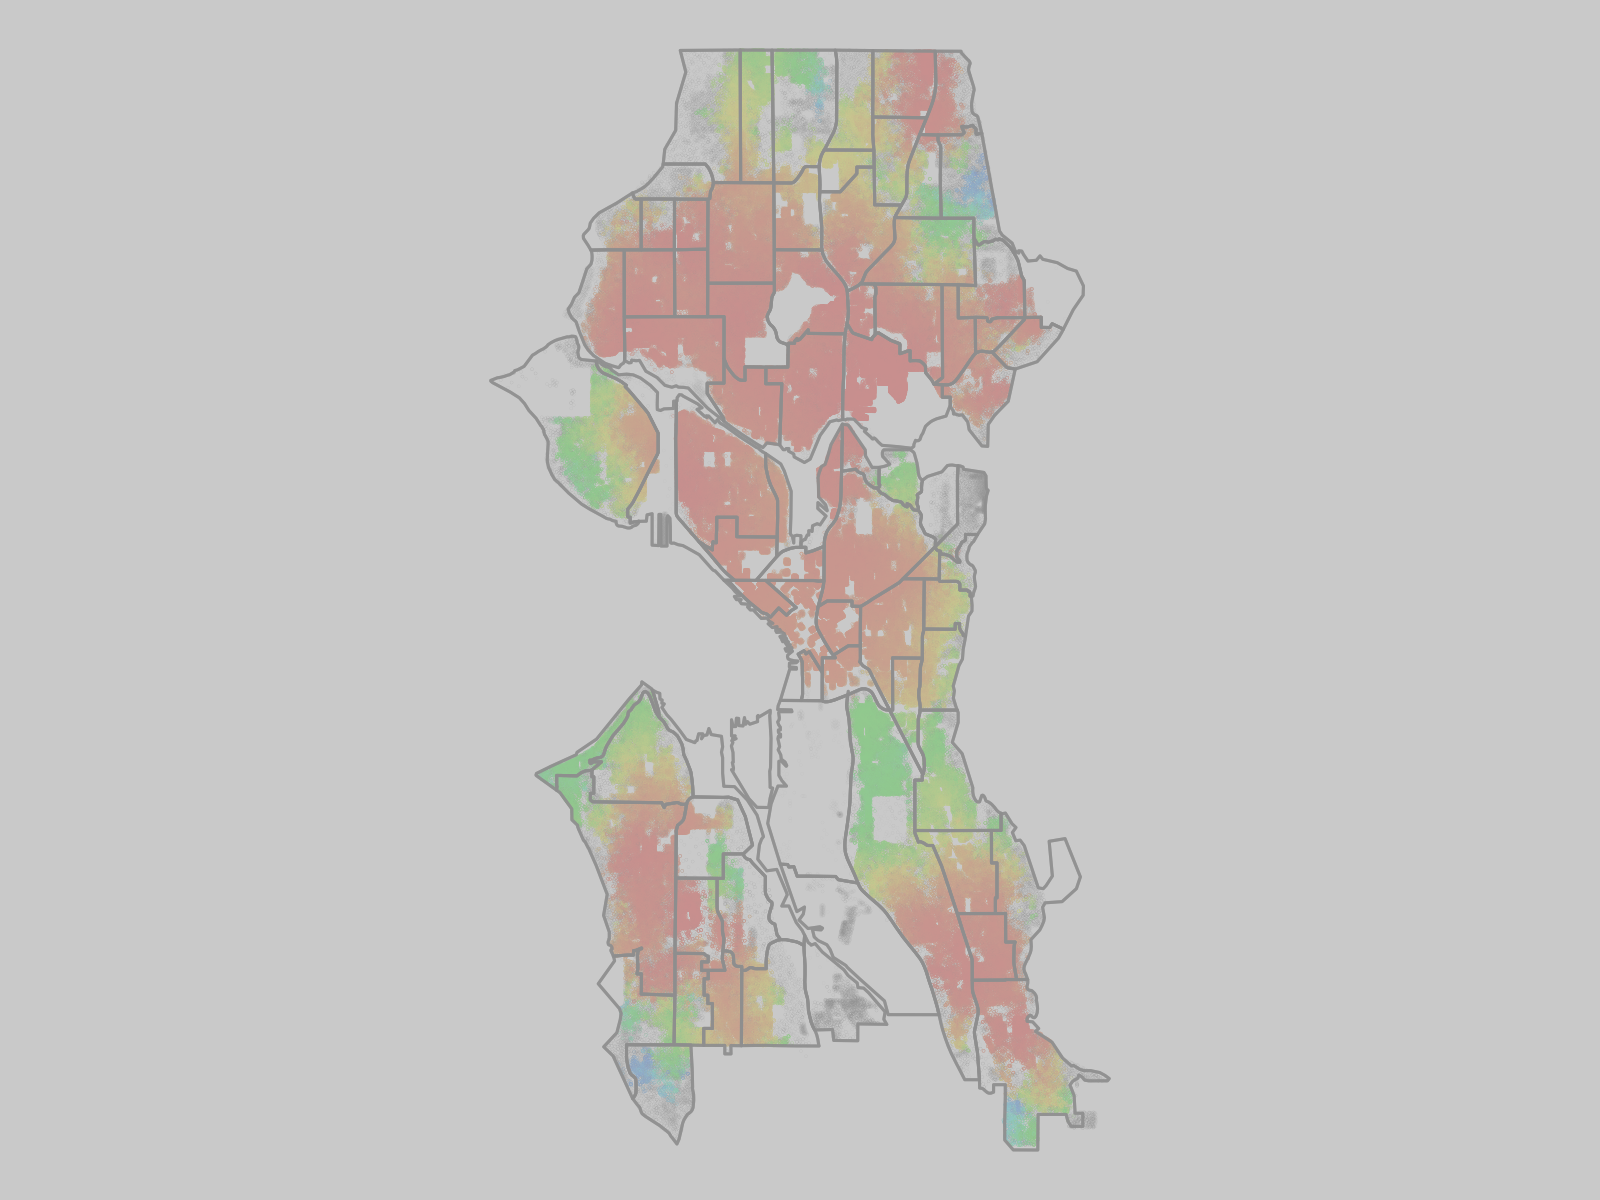
\includegraphics[width=\paperwidth]{graphics/seattle.png}}
\begin{frame}[plain]
  \titlepage
\end{frame}
}

\section[Outline]{}
\begin{frame}[allowframebreaks]{}
\vspace{.5in}
\hspace{.5in}\tableofcontents
\end{frame}




\section{Cluster Sampling}

\begin{frame}{}
\begin{block}{}
\begin{center}
Cluster Sampling
\end{center}
\end{block}
\end{frame}

\subsection{Cluster Sampling Notation}

\begin{frame}{Why Cluster Sampling}
\begin{block}{Common Examples}
\begin{itemize}
\item The population may be widely distributed geographically or may occur in natural clusters (e.g., hh or schools).
\item It may be much less expensive to take a sample of clusters than a SRS of individuals. 
\begin{itemize}
\item Households
\item School districts
\item Schools
\item Classrooms
\item Nursing homes
\item Blocks
\item States
\item Regions
\item Countries
\end{itemize}
\end{itemize}
\end{block}
\end{frame}

\begin{frame}{Notation for Cluster Sampling}
\only<1>{
\begin{block}{PSU Level}
\begin{itemize}
\item $y_{ij}$ = measurement for $j$th element in $i$th psu
\item $N=$ number of ssus in the population
\item $M_i$ = number of ssus in psu $i$
\item $M_0 = \sum_{i=1}^N M_i$ = total number of suss in the population
\item $t_i=\sum_{j=1}^{M_i} y_{ij} =$ total in psu $i$
\item $t=\sum_{i=1}^N t_i = \sum_{i=1}^N \sum_{j=1}^{M_i} y_{ij} $ = population total
\item $S_t^2 = \frac{1}{N-1} \sum_{i=1}^N \left(t_i-\frac{t}{N} \right)^2 =$ population variance of psu totals
\end{itemize}
\end{block}
}
\only<2>{
\begin{block}{SSU level}
\begin{itemize}
\item $\bar{y}_U = \sum_{i=1}^N \sum_{j=1}^{M_i} \frac{y_{ij}}{M_0}=$ population mean
\item $\bar{y}_{iU} =  \sum_{j=1}^{M_i} \frac{y_{ij}}{M_i} = \frac{t_i}{M_i}=$ population mean in psu $i$
\item $S^2 = \sum_{i=1}^N \sum_{j=1}^{M_i}  \frac{(y_{ij}-\bar{y}_U)^2}{M_0-1}=$ population variance (per ssu)
\item $S_i^2 = \sum_{j=1}^{M_i} \frac{(y_{ij}-\bar{y}_{iU})^2}{M_i-1}=$ population variance within psu $i$
\end{itemize}
\end{block}
}
\only<3>{
\begin{block}{Sample Quantities}
\begin{itemize}
\item $y_{ij}$ = measurement for $j$th element in $i$th psu
\item $n=$ number of ssus in the sample
\item $m_i$ = number of ssus in the sample from psu $i$
\item $\bar{y}_i = \sum_{j\in S_i} \frac{y_{ij}}{m_i}$ = sample mean (per ssu) for psu $i$
\item $\hat{t}_i=\sum_{j\in S_i} \frac{M_i}{m_i} y_{ij} =$ estimated total in psu $i$
\item $\hat{t}_{unb}= \sum_{i\in S} \frac{N}{n} \hat{t}_i $ = unbiased estimator of the population total
\item $s_t^2 = \frac{1}{n-1} \sum_{i\in S} \left(t_i-\frac{\hat{t}_{unb}}{N} \right)^2 =$ population variance of psu totals
\item $s_i^2 = \sum_{j \in S_i} \frac{(y_{ij}-\bar{y}_i)^2}{m_i-1}=$ sample variance within psu $i$
\item $w_{ij} =$ sampling weight for ssh $j$ in psu $i$
\end{itemize}
\end{block}
}
\end{frame}


\subsection{One-Stage Cluster Sampling with Fixed M}

\begin{frame}{One-Stage Cluster Sampling}

\begin{textblock*}{100mm}(10mm,0.25\textheight)
\begin{block}{Clusters of Equal Sizes Estimation}
\begin{itemize}
\item $M_i=m_i=M$.
\item This rarely happens in human systems, but is typical of agricultural or industrial problems.
\end{itemize}
\end{block}
\end{textblock*}

\begin{textblock*}{50mm}(65mm,0.5\textheight)
\begin{block}{}
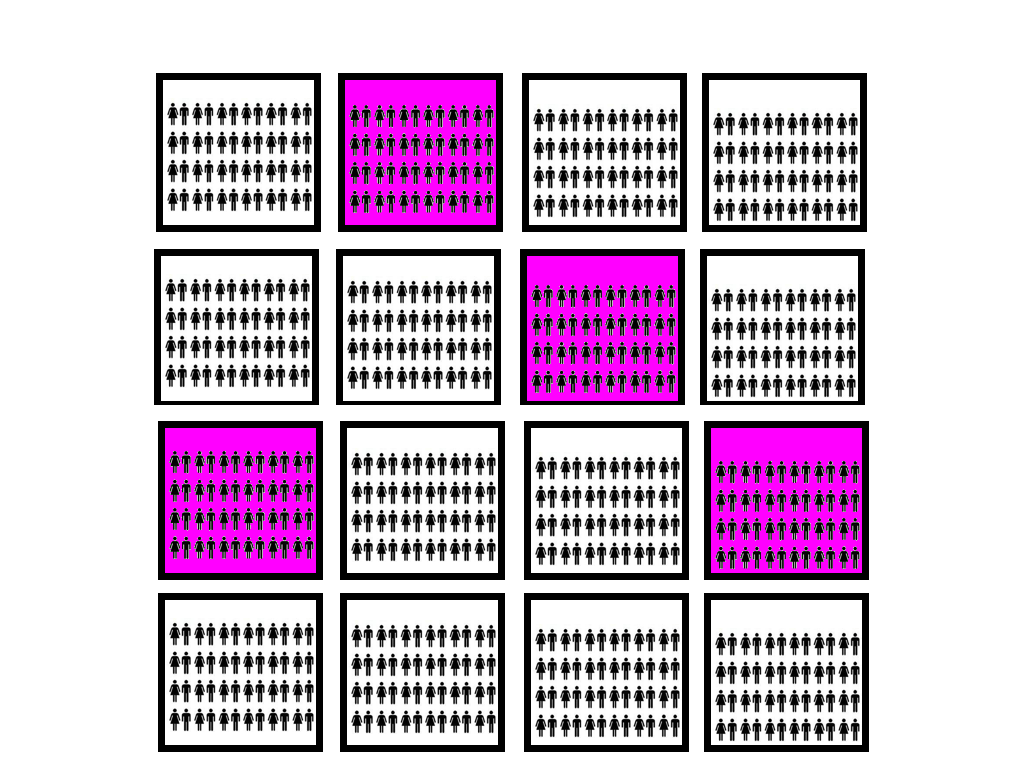
\includegraphics[width=1\linewidth]{figures/clusterEqual.png}
\end{block}
\end{textblock*}

\end{frame}

\begin{frame}{One-Stage Cluster Sampling}
\small
\begin{itemize}
\item We have an SRS of $n$ data points $\{ t_i, i \in S\}$; $t_i$ is the total for all the elements in psi $i$.
$$\hat{t}_S = \sum_{i\in S} \frac{t_i}{n}$$
Estimates the average of the cluster totals.
\item To estimate the total income $t$, we can use the estimator
$$\hat{t}= \frac{N}{n} \sum_{i \in S} t_i$$
\item To make this concrete consider estimating the total income of two person households 
\end{itemize}
\end{frame}


\begin{frame}{One-Stage Cluster Sampling}
\small
\begin{itemize}
\item $V(\hat{t})=N^2 \left(1-\frac{n}{N}\right) \frac{S_t^2}{n}$
\item $SE(\hat{t}) = N\sqrt{ \left(1-\frac{n}{N}\right) \frac{S_t^2}{n}}$
\item $S_t^2$ and $s_t^2$ are the population and sample variance, respectively
\item PSU totals: $$S_t^2 = \frac{1}{N-1} \sum_{i=1}^N \left(t_i-\frac{t}{N}\right)^2$$
and
$$s_t^2 = \frac{1}{n-1} \sum_{i \in S} \left(t_i-\frac{\hat{t}}{N}\right)^2 $$ 
\item $\hat{\bar{y}} = \frac{\hat{t}}{NM}$
\item $V(\hat{\bar{y}}) = \left( 1-\frac{n}{N} \right)\frac{S_t^2}{nM^2}$
\item $SE(\hat{\bar{y}}) = \frac{1}{M}\sqrt{\left(1-\frac{n}{N}\right)\frac{s_t^2}{n}}$
\end{itemize}
\end{frame}


\begin{frame}{One-Stage Cluster Sampling}

\begin{block}{}
\begin{itemize}
\item One-stage cluster sampling with an SRS of psus produces a self-weighting sample.
\item The weight for each observation unit is:
$$w_{ij} = \frac{1}{\Pr(\textrm{ssu $j$ psu is in sample})}=\frac{N}{n}$$
\item $\hat{t} = \sum_{i \in S} \sum_{j \in S_i} w_{ij} y_{ij}$
\item $\hat{\bar{y}} = \frac{\sum_{i \in S} \sum_{j \in S_i} w_{ij} y_{ij}}{\sum_{i \in S} \sum_{j \in S_i} w_{ij}}$
\end{itemize}
\end{block}

\end{frame}

\subsection{Clusters of Equal Sizes: Theory}

\begin{frame}{}
\begin{block}{}
Clusters of Equal Sizes: Theory
\end{block}
\end{frame}

\begin{frame}{Clusters of Equal Sizes: Theory}
\begin{block}{}
\begin{itemize}
\item Goal: Compare \underline{cluster sampling} to \underline{SRS}
\item Note that cluster sampling almost always provides less precision for the estimators than one would obtain by taking an SRS wight he same number of elements!
\end{itemize}
\end{block}
\end{frame}


\begin{frame}{Clusters of Equal Sizes: Theory}
\begin{block}{ANOVA Decomposition}
\begin{itemize}
\item SST=SSB+SSW
\item This corresponds to MST, MSB and MSW
\item Variance of estimators
\begin{itemize}
\item Unlike  \textbf{stratified sampling} where the variances of the estimators depended on the within group variation (MSW), in \textbf{cluster sampling} the variances of the estimators depend on the between group variation (MSB).
\item $F=MSB/MSE$
\begin{itemize}
\item If $F$ is large then stratification $decreases$ variance relative to an SRS
\item If $F$ is large then clustering $increases$ variance relative to an SRS.
%\item If $MSB>MST$  then cluster sampling is less efficient than an SRS.
\end{itemize}
\end{itemize}
\end{itemize}
\end{block}
\end{frame}

\subsection{ICC}

\begin{frame}{Interclass correlation coefficient (ICC)}
\begin{block}{ICC}
\only<1>{
\begin{itemize}
\item Intraclass correlation coefficient (ICC)
\item Intracluster correlation coefficient (ICC)
\item Is a measure on how similar elements in the same cluster are.
\item It provides a measure of \textbf{homogeneity} within the clusters.
\end{itemize}
}
\only<2>{
\begin{itemize}
\item ICC is defined to be the Pearson correlation coefficient for the $NM(M-1)$ pairs $(y_{ij},y_{ik})$ for $i$ between $1$ and $N$ and $j\neq k$.
\item It can be written in terms of the population ANOVA table quantities as:
$$ICC=1-\frac{M}{M-1} \frac{SSW}{SST}$$
\end{itemize}
}
\only<3>{
\begin{itemize}
\item B/c $0\leq SSW/SSTO  \leq1$, it follows that
$$-\frac{1}{M-1} \leq ICC \leq 1$$
\item If the clusters are perfectly homogeneous and hence $SSW=0$ then $ICC=1$
\item $$MSB=\frac{NM-1}{M((N-1)}S^2[1+(M-1)ICC]$$
\item This allows us to say how much precision we lose by taking a cluster sample
$$\frac{V(\hat{t}_{cluster})}{V(\hat{t}_{SRS}} = \frac{MSB}{S^2} = \frac{NM-1}{M(N-1)}[1+(M-1)ICC]$$
\end{itemize}
}
\only<4>{
\begin{itemize}
\item If $N$, the number of psus is in the population, is large
\begin{itemize}
\item $NM-1\approx M(N-1)$ and then the ratio of the variances is approximately $1+(M-1)ICC$
\item $1+(M-1)ICC$ suss taken from a one-stage cluster sample, give us approximately the same amount of information as one ssh from an SRS.
\item If $ICC=0.5$ and $M=5$ then $1+(M-1)ICC=3$, thus we would need 300 elements using cluster sampling to obtain the same precision as an SRS of 100 elements.
\end{itemize}
\end{itemize}
}
\only<5>{
\begin{itemize}
\item $ICC$ is only defined for clusters of equal sizes.
\item An alternative measure of homogeneity in general populations is the adjusted $R^2$, call $R_a^2$ and defined as:
$$R_a^2 = 1- \frac{MSW}{S^2}$$
\item if all psus are of the same size, then the increase in variance due to cluster sampling is:
$$\frac{V(\hat{t}_{cluster})}{V(\hat{t}_{SRS}} = \frac{MSB}{S^2} = 1+\frac{N(M-1)}{N-1}R_a^2$$
\end{itemize}

}
\end{block}
\end{frame}



\subsection{Clusters of Unequal Sizes (One-stage)}

\begin{frame}{}
\begin{block}{}
\begin{center}
Cluster of Unequal Sizes (One-stage)
\end{center}
\end{block}
\end{frame}


\begin{frame}{Clusters of Unequal Sizes (One-stage)}

\begin{textblock*}{100mm}(10mm,0.2\textheight)
\begin{block}{}
In a one-stage cluster sample of $n$ of the $N$ psus, we can estimate population totals and means in two ways:
\begin{itemize}
\item Unbiased Estimation (SRS Theory and census of the cluster)
\item Ratio Estimation
\end{itemize}
\end{block}
\end{textblock*}

\begin{textblock*}{50mm}(10mm,0.5\textheight)
\begin{block}{}
\begin{itemize}
\item Unbiased Estimation
\begin{itemize}
\item $\hat{t}_{unb}=\frac{N}{n} \sum_{i\in S} t_i$
\item $SE(\hat{t}) =N\sqrt{\left(1-\frac{n}{N}\right)\frac{s_t^2}{n}}$
\item $M_0=\sum_{i=1}^N M_i$
\item $\hat{\bar{y}}_{unb} = \hat{t}_{unb}/M_0$
\item $SE(\hat{\bar{y}}_{unb})=SE(\hat{t})/M_0$
\end{itemize}
\end{itemize}
\end{block}
\end{textblock*}


\begin{textblock*}{50mm}(65mm,0.5\textheight)
\begin{block}{}
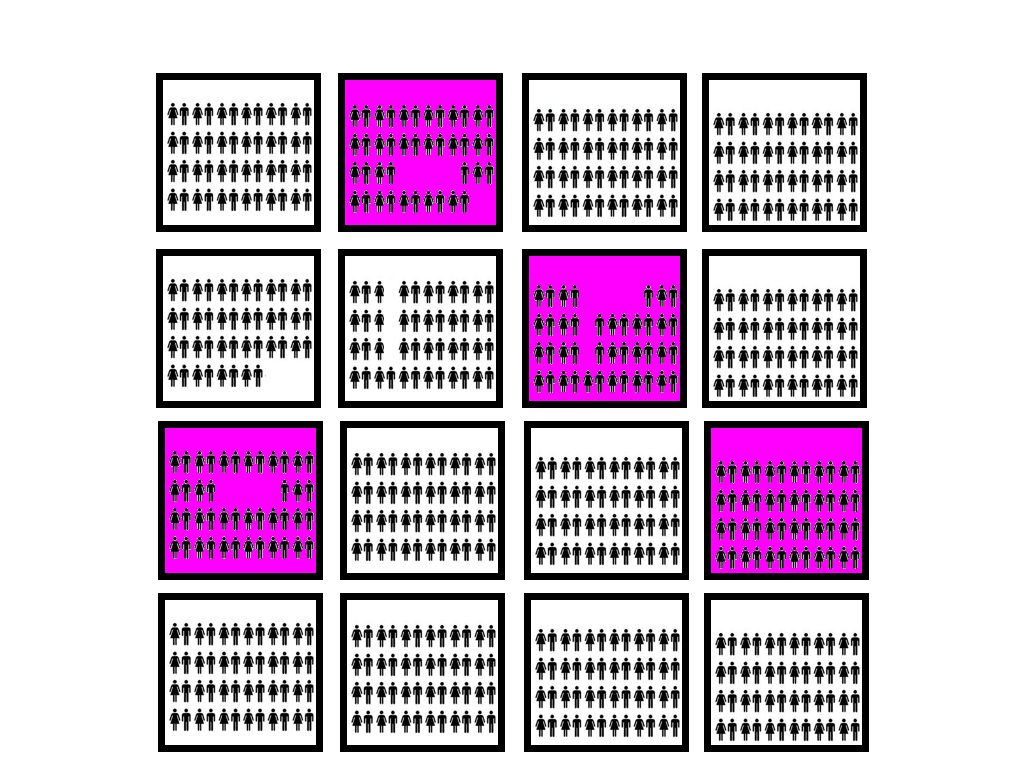
\includegraphics[width=1\linewidth]{figures/cluster.png}
\end{block}
\end{textblock*}

\end{frame}

\begin{frame}{Clusters of Unequal Sizes (One-stage)}
\begin{block}{Sample Weights}
\begin{itemize}
\item The probability that psu is in the sample is $\frac{n}{N}$ (remember this stage is just SRS).
\item B/c this is a one-stage cluster sample, an ssu is included in the sample whenever a psu is included in the sample.
\item $w_{ij} = \frac{1}{\Pr(\textrm{ssu $j$ of psu $i$ is in the sample})} = \frac{N}{n}$
\item Thus One-stage cluster sampling produces a self-weighting sample when psus are selected with equal probabilities.
\item $\hat{t}_{unb} = \sum_{i \in S} \sum_{j \in S_i} w_{ij} y_{ij}$
\end{itemize}
\end{block}
\end{frame}


\subsection{Relationship to Ratio Estimation (One-Stage)}

\begin{frame}{Cluster of Unequal Sizes (One-Stage)}
\begin{block}{Relationship to Ratio Estimation}
\only<1>{
What do we do if $M_0$ is not known?
}
\only<2>{
One solution is the Ratio Estimator!
}
\end{block}

\end{frame}

\begin{frame}{Cluster of Unequal Sizes (One-Stage)}

\only<1>{
\begin{block}{Ratio Estimation: Population}
$$\bar{y}_U =\frac{\sum_{i=1}^N t_i}{\sum_{i=1}^N M_i}=\frac{t}{M_o}$$
\end{block}
}
\only<2-3>{
\begin{block}{Ratio Estimation: Sample}
$$\hat{\bar{y}}_r =\frac{\hat{t}_{unb}}{\hat{M}_0}=\frac{\sum_{i\in S} t_i}{\sum_{i\in S} M_i}=\frac{\sum_{i\in S} M_i \hat{y}_i}{\sum_{i\in S}  M_i}$$
This can be rewritten using the weights $w_{ij}$:
$$\hat{\bar{y}}_r =\frac{\hat{t}_{unb}}{\hat{M}_0}= \frac{\sum_{i \in S} \sum_{j \in S_i} w_{ij} y_{ij}}{\sum_{i \in S} \sum_{j \in S_i} w_{ij}}$$
\end{block}
}
\only<3>{
\begin{block}{}
\begin{align*}
SE(\hat{\bar{y}}_r) &= \sqrt{\left(1-\frac{n}{N} \right)\frac{1}{n\bar{M}^2} \frac{\sum_{i\in S} (t_i-\hat{\bar{y}}_r M_i)^2}{n-1} }\\
&= \sqrt{\left(1-\frac{n}{N} \right)\frac{1}{n\bar{M}^2} \frac{\sum_{i\in S} M_i^2(\bar{y}_i-\hat{\bar{y}}_r )^2}{n-1} }
\end{align*}
\end{block}
}
\only<4>{
\begin{block}{Ratio Estimation: Sample}
\begin{itemize}
\item If we know $M_0$ then we can use ratio estimation to estimate the population total.
\item $\hat{t}_r = M_0 \hat{\bar{y}}_r$ 
\item $SE(\hat{t}_r) =M_0 SE(\hat{t}_r)$
\end{itemize}
\end{block}
}

\end{frame}

\subsection{Two-Stage Cluster Sampling}

\begin{frame}{}
\begin{block}{}
\begin{center}
Two-Stage Cluster Sampling
\end{center}
\end{block}
\end{frame}

\begin{frame}{Two-Stage Cluster Sampling}
\only<1>{
\begin{block}{Comparison}
\begin{itemize}
\item In one-stage cluster sampling you sample PSUs and then take a census of all SSUs.
\item In two-stage cluster sampling you sample PSUs and then take a sample of SSUs.
\item The simplest form is an SRS of PSUs followed by an SRS of SSUs.
\end{itemize}
\end{block}
}
\only<2>{
\begin{block}{Procedure}
\begin{itemize}
\item Select an SRS $S$ of $n$ psus from the population of $N$ psus.
\item Select an SRS of ssus from each selected psu. The SRS of $m_i$ elements from the $i$ psu is denoted $S_i$ and $|S_i|=M_i$.
\end{itemize}
\end{block}
}
\end{frame}

\begin{frame}{Two-Stage Cluster Sampling}

\only<1>{
\begin{block}{One-stage cluster sampling $\hat{t}$}
$$\hat{t}_{unb} = \frac{N}{n} \sum_{i\in S} t_i$$
\end{block}
}

\only<2>{
\begin{block}{Two-stage cluster sampling $\hat{t}$}
\begin{align*}
\hat{t}_i &= \sum_{j \in S_i} \frac{M_i}{m_i} y_{ij} = M_i\bar{y}_i\\
\hat{t}_{unb} &= \frac{N}{n}\sum_{i\in S} \hat{t}_i = \sum{N}{n} \sum_{i\in S} M_i\bar{y}_i = \sum_{i\in S} \sum_{j \in S_i} \frac{N}{n}\frac{M_i}{m_i} y_{ij}
\end{align*}
\end{block}
}
\only<3>{
\begin{block}{Two-stage cluster sampling $\hat{t}$}
\begin{itemize}
\item We can of course rewrite this sum as a weighted sum ...
\item $\Pr(\textrm{ $j$th ssu in $i$th psu is selected })$ = $\Pr(\textrm{ $i$th psu selected})\times \Pr(\textrm{ $j$th ssu selected | $i$th psu selected })$  $=\frac{n}{N} \frac{m_i}{M_i}$
\item Thus $w_{ij}=\frac{NM_i}{nm_i}$ and
\item $\hat{t}_{unb} = \sum_{i\in S} \sum_{j \in S_i} w_{ij} y_{ij}$
\end{itemize}
\end{block}
}
\only<4>{
\begin{block}{Two-stage cluster sampling $SE(\hat{t})$}
$$\hat{V}(\hat{t}_{unb}) = N^2\left(1-\frac{n}{N}\right)\frac{s_t^2}{n}+\frac{N}{n} \sum_{i=1}^N \left(1-\frac{m_i}{M_i}\right)M_i^2 \frac{s_i^2}{m_i}$$
\begin{itemize}
\item $s_t^2= \frac{1}{n-1} \sum_{i \in S} \left(\hat{t}_i-\frac{\hat{t}_{unb}}{N} \right)^2$
\item $s_i^2=\frac{1}{m_i-1} \sum_{j\in S_i} \sum_{j\in S_i} (y_{ij}-\bar{y}_i)^2$
\end{itemize}
\end{block}
}
\only<4>{
\begin{block}{Two-stage cluster sampling $\hat{\bar{y}}_{unb}$}
$$\hat{\bar{y}}_{unb} = \hat{t}_{unb}/M_0$$
$$SE(\hat{\bar{y}}_{unb})=SE(\hat{t}_{unb})/M_0$$
\end{block}
}
\only<5>{
\begin{block}{Two-stage cluster sampling $\hat{\bar{y}}_{r}$}
$$\hat{\bar{y}}_{r} =
\frac{\sum_{i \in S} \hat{t}_i}{\sum_{i \in S} M_i} = \frac{\sum_{i \in S} M_i \bar{y}_i}{\sum_{i \in S} M_i}
 $$
$$\hat{V}(\hat{\bar{y}}_{r}) = \frac{1}{\bar{M}^2}\left(1-\frac{n}{N}\right)\frac{s_r^2}{n}+\frac{1}{nN\bar{M}^2} \sum_{i\in S} M_i^2\left(1-\frac{m_i}{M_i} \right)\frac{s_i^2}{m_i}$$
where $s_r^2=\frac{1}{n-1} \sum_{i\in S} (M_i\bar{y}_i-M_i\hat{\bar{y}}_r)^2$
\end{block}
}
\end{frame}





\begin{frame}[containsverbatim]{Example: coot}
\begin{itemize}
\item Arnold's (1991) work on egg size and volume of American Coot eggs in Minnedosa, Manitoba.
\item We are looking at the volumes of a subsample of eggs in clutches (nests of eggs) with at least two eggs available for measurement.
\end{itemize}
\small
\begin{knitrout}
\definecolor{shadecolor}{rgb}{1, 1, 1}\color{fgcolor}\begin{kframe}
\begin{alltt}
\hlcom{# devtools::install_github('SSDALab/lohrData')}
\hlkwd{library}\hlstd{(lohrData)}
\hlkwd{data}\hlstd{(coots)}
\hlkwd{head}\hlstd{(coots)}
\end{alltt}
\begin{verbatim}
 R >    CLUTCH CSIZE LENGTH BREADTH    VOLUME TMT
 R >  1      1    13  44.30   31.10 3.7957569   1
 R >  2      1    13  45.90   32.70 3.9328497   1
 R >  3      2    13  49.20   34.40 4.2156036   1
 R >  4      2    13  48.70   32.70 4.1727621   1
 R >  5      3     6  51.05   34.25 0.9317646   0
 R >  6      3     6  49.35   34.40 0.9007362   0
\end{verbatim}
\end{kframe}
\end{knitrout}
\end{frame}


\begin{frame}[containsverbatim]{Example: coot}
\tiny
\begin{center}
\begin{knitrout}
\definecolor{shadecolor}{rgb}{1, 1, 1}\color{fgcolor}\begin{kframe}
\begin{alltt}
\hlkwd{plot}\hlstd{(coots}\hlopt{$}\hlstd{CLUTCH, coots}\hlopt{$}\hlstd{VOLUME,} \hlkwc{pch} \hlstd{=} \hlnum{19}\hlstd{,} \hlkwc{cex} \hlstd{=} \hlnum{0.5}\hlstd{)}
\end{alltt}
\end{kframe}

{\centering 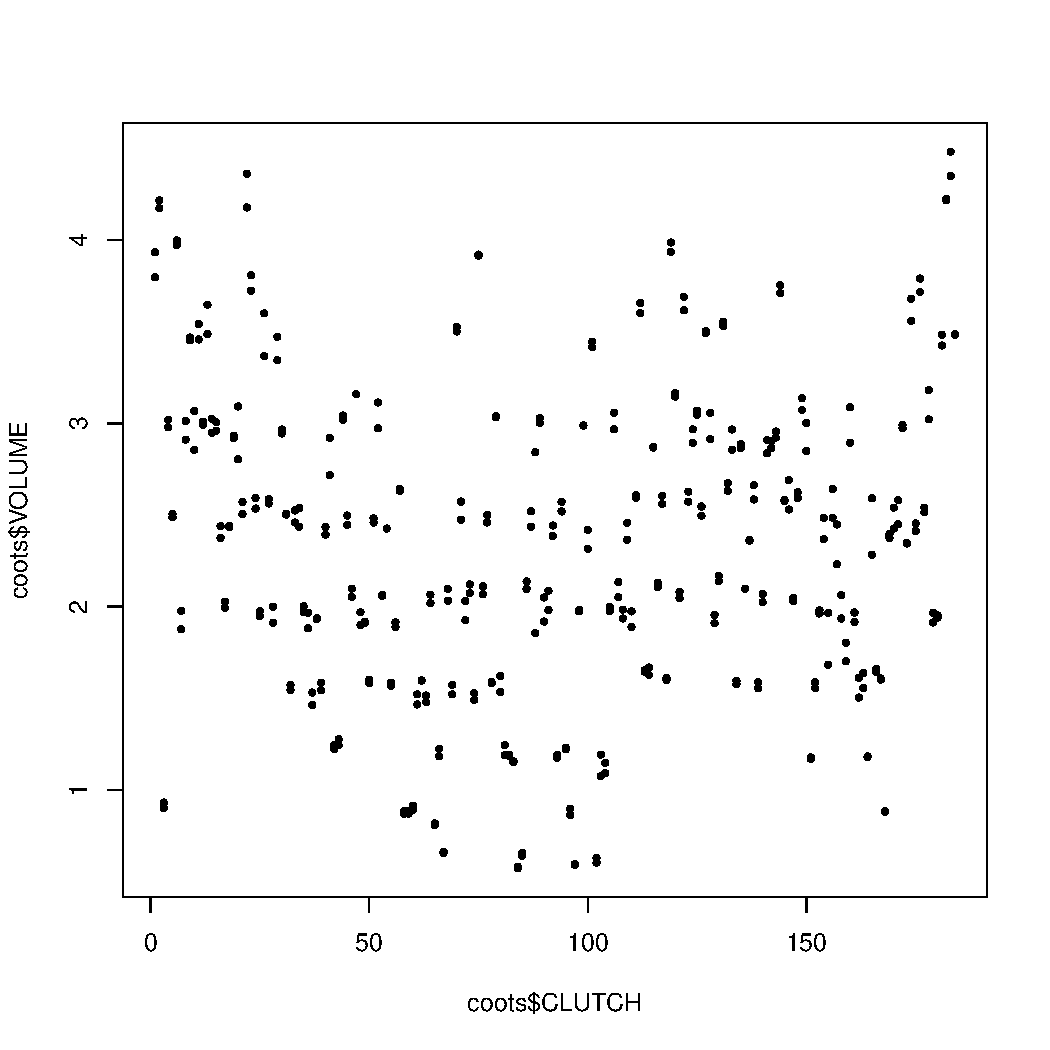
\includegraphics[width=.7\linewidth]{figure/unnamed-chunk-3-1} 

}


\end{knitrout}
\end{center}
\end{frame}

\begin{frame}[containsverbatim]{Example: coot}
\small
\begin{center}
\begin{knitrout}
\definecolor{shadecolor}{rgb}{1, 1, 1}\color{fgcolor}\begin{kframe}
\begin{alltt}
\hlstd{foo} \hlkwb{<-} \hlkwd{split}\hlstd{(coots}\hlopt{$}\hlstd{VOLUME, coots}\hlopt{$}\hlstd{CLUTCH)}
\hlcom{# foo[[1]]}
\hlstd{ybari} \hlkwb{<-} \hlkwd{sapply}\hlstd{(foo, mean)}

\hlstd{o} \hlkwb{<-} \hlkwd{order}\hlstd{(ybari)}
\hlstd{one} \hlkwb{<-} \hlkwd{sapply}\hlstd{(foo,} \hlstr{"["}\hlstd{,} \hlnum{1}\hlstd{)}
\hlstd{two} \hlkwb{<-} \hlkwd{sapply}\hlstd{(foo,} \hlstr{"["}\hlstd{,} \hlnum{2}\hlstd{)}
\hlkwd{plot}\hlstd{(}\hlnum{1}\hlopt{:}\hlkwd{length}\hlstd{(o), one[o],} \hlkwc{pch} \hlstd{=} \hlnum{19}\hlstd{,} \hlkwc{cex} \hlstd{=} \hlnum{0.1}\hlstd{)}
\hlkwd{points}\hlstd{(}\hlnum{1}\hlopt{:}\hlkwd{length}\hlstd{(o), two[o],} \hlkwc{pch} \hlstd{=} \hlnum{19}\hlstd{,} \hlkwc{cex} \hlstd{=} \hlnum{0.1}\hlstd{)}

\hlkwa{for} \hlstd{(i} \hlkwa{in} \hlnum{1}\hlopt{:}\hlkwd{length}\hlstd{(o))} \hlkwd{segments}\hlstd{(}\hlkwc{x0} \hlstd{= i,} \hlkwc{x1} \hlstd{= i,} \hlkwc{y0} \hlstd{= one[o[i]],}
    \hlkwc{y1} \hlstd{= two[o[i]],} \hlkwc{cex} \hlstd{=} \hlnum{1}\hlstd{)}
\end{alltt}
\end{kframe}
\end{knitrout}
\end{center}
\end{frame}

\begin{frame}[containsverbatim]{Example: coot}
\small
\begin{center}

\begin{knitrout}
\definecolor{shadecolor}{rgb}{1, 1, 1}\color{fgcolor}

{\centering 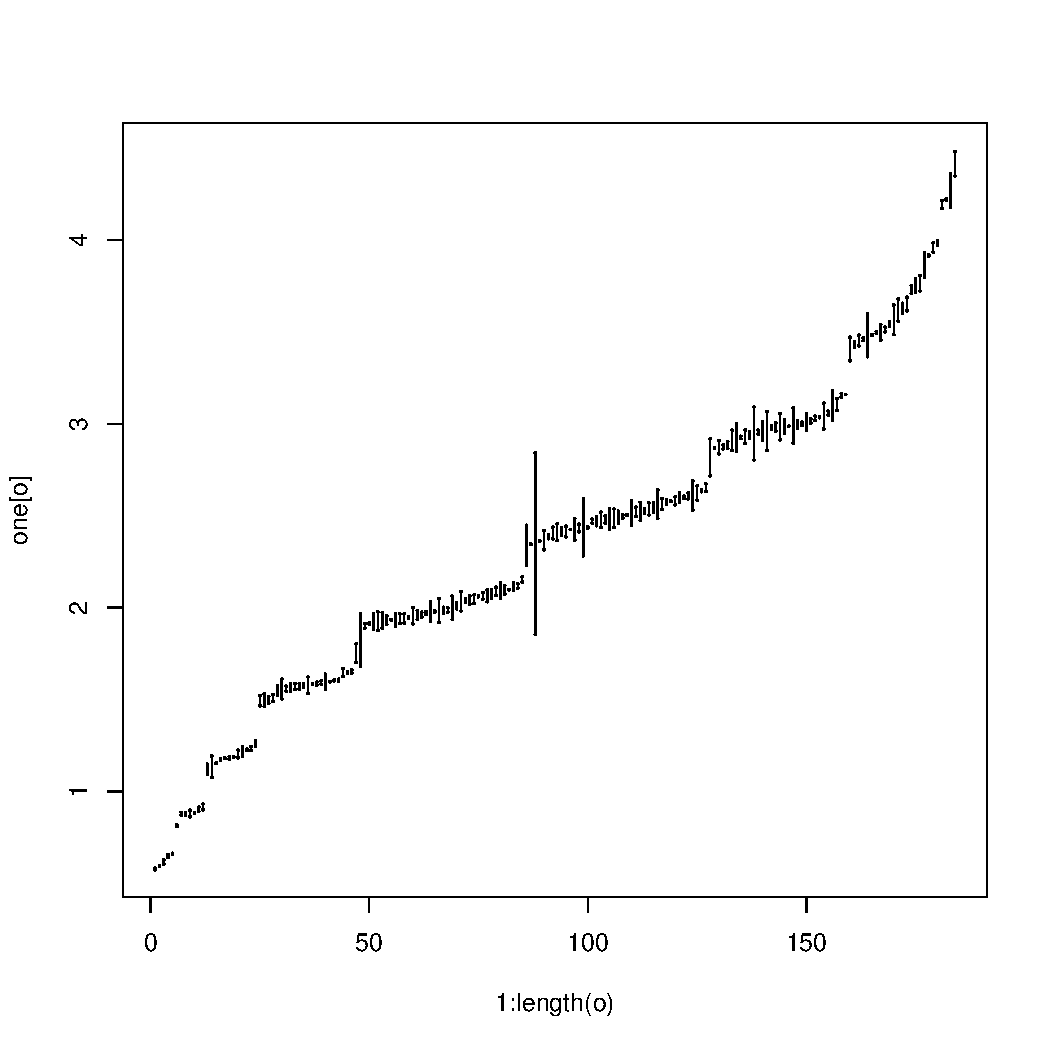
\includegraphics[width=.7\linewidth]{figure/unnamed-chunk-5-1} 

}


\end{knitrout}
\end{center}
\end{frame}

\begin{frame}[containsverbatim]{Example: coot}
\tiny
\begin{knitrout}
\definecolor{shadecolor}{rgb}{1, 1, 1}\color{fgcolor}\begin{kframe}
\begin{alltt}
\hlstd{foo} \hlkwb{<-} \hlkwd{split}\hlstd{(coots}\hlopt{$}\hlstd{VOLUME, coots}\hlopt{$}\hlstd{CLUTCH)}
\hlstd{ybari} \hlkwb{<-} \hlkwd{sapply}\hlstd{(foo, mean)}
\hlstd{si2} \hlkwb{<-} \hlkwd{sapply}\hlstd{(foo, var)}
\hlstd{Mi} \hlkwb{<-} \hlkwd{sapply}\hlstd{(}\hlkwd{split}\hlstd{(coots}\hlopt{$}\hlstd{CSIZE, coots}\hlopt{$}\hlstd{CLUTCH), mean)}
\hlstd{hat.ti} \hlkwb{<-} \hlstd{(Mi}\hlopt{/}\hlnum{2}\hlstd{)} \hlopt{*} \hlkwd{sapply}\hlstd{(foo, sum)}
\hlstd{ssufpc} \hlkwb{<-} \hlstd{(}\hlnum{1} \hlopt{-} \hlnum{2}\hlopt{/}\hlstd{Mi)}
\hlstd{ybar.r} \hlkwb{<-} \hlkwd{sum}\hlstd{(hat.ti)}\hlopt{/}\hlkwd{sum}\hlstd{(Mi)}

\hlstd{var1} \hlkwb{<-} \hlstd{ssufpc} \hlopt{*} \hlstd{(Mi}\hlopt{^}\hlnum{2}\hlstd{)} \hlopt{*} \hlstd{(si2}\hlopt{/}\hlnum{2}\hlstd{)}
\hlstd{var2} \hlkwb{<-} \hlstd{(hat.ti} \hlopt{-} \hlstd{Mi} \hlopt{*} \hlstd{ybar.r)}\hlopt{^}\hlnum{2}

\hlstd{cluster.table} \hlkwb{<-} \hlkwd{data.frame}\hlstd{(}\hlkwc{Clutch} \hlstd{=} \hlnum{1}\hlopt{:}\hlnum{184}\hlstd{, Mi, ybari, si2,}
    \hlstd{hat.ti, var1, var2)}
\hlkwd{head}\hlstd{(cluster.table)}
\end{alltt}
\begin{verbatim}
 R >    Clutch Mi     ybari          si2    hat.ti
 R >  1      1 13 3.8643033 0.0093972179 50.235943
 R >  2      2 13 4.1941828 0.0009176971 54.524377
 R >  3      3  6 0.9162504 0.0004813808  5.497502
 R >  4      4 11 2.9983346 0.0007950278 32.981681
 R >  5      5 10 2.4957075 0.0001574425 24.957075
 R >  6      6 13 3.9842595 0.0003303709 51.795373
 R >          var1         var2
 R >  1 0.67190108 3.189232e+02
 R >  2 0.06561534 4.904832e+02
 R >  3 0.00577657 8.922633e+01
 R >  4 0.03935387 3.119577e+01
 R >  5 0.00629770 2.630604e-03
 R >  6 0.02362152 3.770530e+02
\end{verbatim}
\end{kframe}
\end{knitrout}
\end{frame}

\begin{frame}[containsverbatim]{Example: coot}
\tiny
\begin{knitrout}
\definecolor{shadecolor}{rgb}{1, 1, 1}\color{fgcolor}\begin{kframe}
\begin{alltt}
\hlstd{ybar.r}
\end{alltt}
\begin{verbatim}
 R >  [1] 2.490579
\end{verbatim}
\begin{alltt}
\hlstd{sr2} \hlkwb{<-} \hlstd{(}\hlnum{1}\hlopt{/}\hlstd{(}\hlnum{183}\hlstd{))} \hlopt{*} \hlkwd{sum}\hlstd{(var2)}
\hlstd{sr2}
\end{alltt}
\begin{verbatim}
 R >  [1] 62.51136
\end{verbatim}
\begin{alltt}
\hlcom{### Why no fpc? is this justified?}
\hlstd{vhat.ybar.r.nfpc} \hlkwb{<-} \hlstd{(}\hlnum{1}\hlopt{/}\hlstd{(}\hlkwd{mean}\hlstd{(Mi)}\hlopt{^}\hlnum{2}\hlstd{))} \hlopt{*} \hlstd{sr2}\hlopt{/}\hlnum{184}
\hlstd{se.ybar.r.nfpc} \hlkwb{<-} \hlkwd{sqrt}\hlstd{(vhat.ybar.r.nfpc)}
\hlstd{se.ybar.r.nfpc}
\end{alltt}
\begin{verbatim}
 R >  [1] 0.0610403
\end{verbatim}
\begin{alltt}
\hlstd{CV.hat} \hlkwb{<-} \hlstd{se.ybar.r.nfpc}\hlopt{/}\hlstd{ybar.r}
\hlstd{CV.hat}
\end{alltt}
\begin{verbatim}
 R >  [1] 0.02450848
\end{verbatim}
\end{kframe}
\end{knitrout}
\end{frame}

\section{Unequal-Probability Sampling}
\begin{frame}{}
\begin{block}{}
Unequal-Probability Sampling
\end{block}
\end{frame}

\begin{frame}{Unequal-Probability Sampling}
\begin{itemize}
\item Sometimes it is not practical or desirable to sample every cluster or unit with equal probability.
\item Theory and estimators in this framework have been developed for \textbf{with} and \textbf{without} replacement.
\item Theory \textbf{with} replacement is slightly easier, in the sense that the estimates and sampling procedures are simpler.
\item Without replacement is more efficient then with replacement.
\item You should read Section 6.0-6.4. Here we will only cover Unequal-probability sampling without replacement.
\end{itemize}
\end{frame}

\section{Probability Proportional to Size (PPS)}

\begin{frame}{}
\begin{block}{}
\begin{center}
Probability Proportional to Size (PPS)
\end{center}
\end{block}
\end{frame}

\begin{frame}{Probability Proportional to Size (PPS)}
\begin{block}{With-replacement Estimation}
\only<1>{
\begin{itemize}
\item $\Pr(\textrm{unit $i$ selected on first draw})=\psi_i$
\item $\Pr(unit $i$ in sample)=\pi_i$
\item One-stage Sampling with replacement: $\psi=\Pr(\textrm{select unit $i$ on first draw})$
\item $\hat{t}_\psi = \frac{1}{n} \sum_{i \in R} \frac{t_i}{\psi_i} = \frac{1}{n}\sum_{i\in R} u_i =\bar{u}$
\item $\hat{V} (\hat{t}_\psi) =\frac{s_u^2}{n} = \frac{1}{n}\frac{1}{n-1} \sum_{i \in R} (u_i-\bar{u})^2=\frac{1}{n}\frac{1}{n-1} \sum_{i \in R}  \left( \frac{t_i}{\psi}-\hat{t}_\psi \right)^2$
\item This is known as the Hansen-Hurwitz (1943) Estimator.
\end{itemize}
}
\only<2>{
\begin{itemize}
\item We designing selection probabilities, one wants to choose the $\psi_i$'s so that the variance of $\hat{t}_\psi$ is as small as possible.
\item Ideally we would choose $\psi_i=t_i/t$ and $\hat{t}_\psi=t$ for all samples and $V(\hat{t}_\psi)=0$.
\item In practice this is not possible, or we are interested in more than a single total from a survey.
\item It is common to take $\psi$ to be proportion of the elements in psu $i$ or the relative size of psu $i$.
\item With $M_i$ the number of elements in the $i$th psu and $M_0=\sum_{i=1}^N M_i$ the number of elements in the population.
\item We take $\psi_i=M_i/M_0$.
\item This choice of $\psi_i$ is called \textbf{probability proportional to size (pps)}
\end{itemize}
}
\only<3>{
\begin{itemize}
\item Thus for one-stage ops sampling $t_i/\psi_i = t_iM_o/M_i = M_0\bar{y}_i$
\item $\hat{t}_\psi=\frac{1}{n} \sum_{i \in R} M_0 \bar{y}_i$
\item $\hat{\bar{y}}_\psi = \frac{1}{n} \sum_{i \in R} \bar{y}_i$ with $\psi=M_i/M_0$
\item $\hat{\bar{y}}_\psi $ is the average of the sampled psu means.
\item $\hat{V}(\hat{\bar{y}}_\psi ) = \frac{1}{n}\frac{1}{n-1} \sum_{i \in R} (\bar{y}_i-\hat{\bar{y}}_\psi )^2$
\end{itemize}

}
\end{block}
\end{frame}

\begin{frame}[containsverbatim]{}

\tiny
\begin{knitrout}
\definecolor{shadecolor}{rgb}{1, 1, 1}\color{fgcolor}\begin{kframe}
\begin{alltt}
\hlkwd{library}\hlstd{(lohrData)}
\hlkwd{data}\hlstd{(statepop)}
\hlkwd{head}\hlstd{(statepop)}
\end{alltt}
\begin{verbatim}
 R >    STATE      COUNTY LANDAREA    POPN PHYS FARMPOP
 R >  1    AL      Wilcox      889   13672    4     666
 R >  2    AZ    Maricopa     9204 2209567 4320    2124
 R >  3    AZ    Maricopa     9204 2209567 4320    2124
 R >  4    AZ       Pinal     5370  120786   61     881
 R >  5    AR     Garland      678   76100  131     524
 R >  6    AR Mississippi      898   55060   48     955
 R >    NUMFARM FARMACRE VETERANS PERCVIET
 R >  1     322   156950      836     20.8
 R >  2    2334  1391456   262170     31.5
 R >  3    2334  1391456   262170     31.5
 R >  4     730  1958489    14858     29.1
 R >  5     389    41293    11055     21.3
 R >  6     615   488042     5285     33.8
\end{verbatim}
\end{kframe}
\end{knitrout}
\end{frame}


\begin{frame}[containsverbatim]{}
\tiny
\begin{knitrout}
\definecolor{shadecolor}{rgb}{1, 1, 1}\color{fgcolor}\begin{kframe}
\begin{alltt}
\hlstd{M0} \hlkwb{<-} \hlnum{255077536}
\hlstd{totalCounty} \hlkwb{<-} \hlkwd{data.frame}\hlstd{(}\hlkwc{state} \hlstd{= statepop}\hlopt{$}\hlstd{STATE,} \hlkwc{county} \hlstd{= statepop}\hlopt{$}\hlstd{COUNTY,}
    \hlkwc{popsize} \hlstd{= statepop}\hlopt{$}\hlstd{POPN,} \hlkwc{psi} \hlstd{= statepop}\hlopt{$}\hlstd{POPN}\hlopt{/}\hlstd{(M0),} \hlkwc{numPhys} \hlstd{= statepop}\hlopt{$}\hlstd{PHYS,}
    \hlkwc{ti_psi} \hlstd{= statepop}\hlopt{$}\hlstd{PHYS}\hlopt{/}\hlstd{(statepop}\hlopt{$}\hlstd{POPN}\hlopt{/}\hlstd{M0))}
\end{alltt}
\end{kframe}
\end{knitrout}
\end{frame}

\begin{frame}[containsverbatim]{}

\tiny
\begin{knitrout}
\definecolor{shadecolor}{rgb}{1, 1, 1}\color{fgcolor}\begin{kframe}
\begin{alltt}
\hlkwd{head}\hlstd{(totalCounty)}
\end{alltt}
\begin{verbatim}
 R >    state      county popsize          psi numPhys
 R >  1    AL      Wilcox   13672 5.359939e-05       4
 R >  2    AZ    Maricopa 2209567 8.662335e-03    4320
 R >  3    AZ    Maricopa 2209567 8.662335e-03    4320
 R >  4    AZ       Pinal  120786 4.735266e-04      61
 R >  5    AR     Garland   76100 2.983407e-04     131
 R >  6    AR Mississippi   55060 2.158559e-04      48
 R >       ti_psi
 R >  1  74627.72
 R >  2 498710.81
 R >  3 498710.81
 R >  4 128820.64
 R >  5 439095.36
 R >  6 222370.54
\end{verbatim}
\end{kframe}
\end{knitrout}
\end{frame}

\begin{frame}[containsverbatim]{}

\tiny
\begin{knitrout}
\definecolor{shadecolor}{rgb}{1, 1, 1}\color{fgcolor}\begin{kframe}
\begin{alltt}
\hlcom{### Table Descriptives}
\hlkwd{sum}\hlstd{(totalCounty}\hlopt{$}\hlstd{ti_psi)}
\end{alltt}
\begin{verbatim}
 R >  [1] 57030430
\end{verbatim}
\begin{alltt}
\hlkwd{sd}\hlstd{(totalCounty}\hlopt{$}\hlstd{ti_psi)}\hlopt{/}\hlkwd{sqrt}\hlstd{(}\hlnum{100}\hlstd{)}
\end{alltt}
\begin{verbatim}
 R >  [1] 41401.23
\end{verbatim}
\begin{alltt}
\hlcom{## n}
\hlkwd{nrow}\hlstd{(totalCounty)}
\end{alltt}
\begin{verbatim}
 R >  [1] 100
\end{verbatim}
\begin{alltt}
\hlcom{## Sum of weights}
\hlkwd{sum}\hlstd{(M0}\hlopt{/}\hlstd{totalCounty}\hlopt{$}\hlstd{popsize)}
\end{alltt}
\begin{verbatim}
 R >  [1] 245072
\end{verbatim}
\end{kframe}
\end{knitrout}
\end{frame}


\subsection{Unequal-Probability Sampling Without Replacement}

\begin{frame}{}
\begin{block}{}
\begin{center}
Unequal-Probability Sampling Without Replacement
\end{center}
\end{block}
\end{frame}

\begin{frame}{Unequal-Probability Sampling Without Replacement}

\begin{block}{The Horvitz-Thompson Estimator for One-stage}
\only<1>{
\begin{itemize}
\item Assume we have a without-replacement sample of $n$ psus, and we know the inclusion probability
$$\pi_i=\Pr(\textrm{ unit $i$ in sample}).$$
\item The joint inclusion probability $$\pi_{ik} = \Pr(\textrm{ units $i$ and $k$ are both in the sample}).$$
\item The inclusion probability $\pi_i$ can be calculated as the sum of the probabilities of all sample containing the $i$th unit and has the property $$\sum_{i=1}^N\pi_i=n.$$
%\item For the $\pi_{ik}$'s, $$\sum_{k=1\\k\neq1}^N \pi_{ik} = (n-1)\pi_i.$$
\end{itemize}
}
\only<2>{
\begin{itemize}
\item For the $\pi_{ik}$'s, $$\sum_{\substack{k=1\\ k\neq1}}^N \pi_{ik} = (n-1)\pi_i.$$
\end{itemize}
}
\only<3>{
\begin{itemize}
\item B/c the inclusion probabilities sum to $n$, we can think of $$\pi_i/n$$ as the ``average probability" that a unit will be selected on one of the draws.
\end{itemize}
}
\only<4>{
\begin{itemize}
\item The \textbf{Horvitz-Thompson (HT) estimator} of the population total:
$$\hat{t}_{HT} = \sum_{i \in S} \frac{t_i}{\pi_i} = \sum_{i=1}^N Z_i \frac{t_i}{\pi_i}$$
where $Z_i=1$ if psu $i$ is in the sample, and $0$ otherwise.
\item The HT estimator is unbiased, i.e.,
$$E[\hat{T}_{HT}] =  \sum_{i=1}^N \pi_i \frac{t_i}{\pi_i} = t.$$
\end{itemize}
}
\only<5>{
\begin{itemize}
\item The Variance for the HT (One-stage) Cluster Sample is:
\begin{align*}
V(\hat{t}_{HT}) &= \sum_{i=1}^N \frac{1-\pi_i}{\pi_i} t_i^2 + \sum_{i=1}^N\sum_{k\neq i}^N \frac{\pi_{ik}-\pi_i\pi_k}{\pi_i\pi_k} t_it_k\\
&= \frac{1}{2} \sum_{i=1}^N\sum_{\substack{k=1\\ k\neq i}}^N (\pi_i\pi_k-\pi_{ik})\left( \frac{t_i}{\pi_i} - \frac{t_k}{\pi_k}\right)^2.
\end{align*}
\item You can see that the variance of the HT estimator is 0 if $t_i$ is proportional to $\pi_i$.
\end{itemize}
}

\only<6>{
\begin{itemize}
\item The Estimated Variance for the HT (One-stage) Cluster Sample is:
\begin{align*}
\hat{V}_{HT}(\hat{t}_{HT}) &= \sum_{i\in S} (1-\pi_i)\frac{t_i^2}{\pi_i^2} + \sum_{i \in S} \sum_{\substack{k\in S\\ k\neq i}} \frac{\pi_{ik}-\pi_i\pi_k}{\pi_{ik}} \frac{t_i}{\pi_i}\frac{t_k}{\pi_k}.
\end{align*}
\item An alternative estimator proposed by Sen-Yates-Grundy (SYG) for the variance:
$$\hat{V}_{SYG}(\hat{t}_{HT}) = \frac{1}{2} \sum_{i\in S}\sum_{\substack{k\in S\\ k\neq i}} \frac{\pi_i\pi_k-\pi_{ik}}{\pi_{ik}}\left( \frac{t_i}{\pi_i} - \frac{t_k}{\pi_k}\right)^2$$ 
\end{itemize}
}

\end{block}

\end{frame}

\subsection{Cluster Sampling Unequal-Probability Sampling (Two-Stage)}

\begin{frame}{}
\begin{block}{}
\begin{center}
Cluster Sampling Unequal-Probability Sampling (Two-Stage)
\end{center}
\end{block}
\end{frame}

\begin{frame}{Cluster Sampling Unequal-Probability Sampling (Two-Stage)}
\begin{block}{Horvitz-Thompson for Two Stage}
\only<1>{
$$\hat{t}_{HT} = \sum_{i \in S} \frac{\hat{t}_i}{\pi_i} = \sum_{i=1}^N Z_i \frac{\hat{t}_i}{\pi_i}$$
Where $Z_i=1$ if psu $i$ is in the sample, and 0 otherwise.

\begin{itemize}
\item The two-stag Horvitz-Thompson estimator is an unbiased estimator of $t$ as long as $E[\hat{t}_i]=t_i$ for each psu $i$.
\end{itemize}
}
\only<2>{
\begin{itemize}
\item The variance of the HT Two-Stage estimator: 
\begin{align*}
V(\hat{t}_{HT}) &= \sum_{i=1}^N \frac{1-\pi_i}{\pi_i}t_i^2 + \sum_{i=1}^N \sum_{k\neq i}^N \frac{\pi_{ik}-\pi_i\pi_k}{\pi_i\pi_k}t_it_k+\sum_{i=1}^N \frac{V(\hat{t}_i)}{\pi_i}\\
&= \frac{1}{2} \sum_{i =1}^N \sum_{\substack{k= 1 \\ k\neq i}}^N (\pi_i\pi_k-\pi_{ik})\left(\frac{t_i}{\pi_i}-\frac{t_k}{\pi_k}\right)^2+\sum_{i=1}^N \frac{V(\hat{t}_i)}{\pi_i}
\end{align*}
\end{itemize}
}
\only<3>{
\begin{itemize}
\item The estimated variance of the HT Two-Stage estimator: 

\begin{align*}
\hat{V}_{HT}(\hat{t}_{HT}) &= \sum_{i\in S} (1-\pi_i)\frac{\hat{t}_i^2}{\pi_i^2}+\sum_{i\in S} \sum_{\substack{k\in S\\ k\neq i}} \frac{\pi_{ik}-\pi_i\pi_k}{\pi_{ik}}\frac{\hat{t}_i}{\pi_i}\frac{\hat{t}_k}{\pi_k}+\sum_{i\in S} \frac{V(\hat{t}_i)}{\pi}\\
\hat{V}_{SYG} (\hat{t}_{HT}) &= \frac{1}{2}\sum_{i\in S} \sum_{\substack{k\in S\\ k\neq i}} \frac{\pi_{ik}-\pi_i\pi_k}{\pi_{ik}} \left( \frac{\hat{t}_i}{\pi_i}-\frac{\hat{t}_k}{\pi_k} \right)^2+\sum_{i\in S} \frac{V(\hat{t}_i)}{\pi}
\end{align*}

\begin{itemize}
\item Both estimators are unbiased, however they can be negative in practice.
\end{itemize}

\end{itemize}
}

\end{block}

\end{frame}




\end{document}
%%%




\section{Sample Size Calculations}
\begin{frame}{Determining Sample Sizes}
\begin{itemize}
\item Assume a stratified sample:
\item $\hat{t}_{yrc} = \hat{B}t_x$
\item $\hat{B} = \frac{\hat{t}_{y,str}}{\hat{t}_{x,str}}$
\item $\hat{t}_{y,str} = \sum_{h=1}^H N_h \bar{y}_h=\sum_{h=1}^H \sum_{j\in S_h} w_{hj}y_{hj}$, where $$w_{hj}=N_h/n_h$
\item $\hat{t}_{x,str} = \sum_{h=1}^H N_h \bar{x}_h=\sum_{h=1}^H \sum_{j\in S_h} w_{hj}x_{hj}$
\end{itemize}

\end{frame}

\begin{frame}[containsverbatim]{}
\small

\end{frame}



%%%%%%%%%%%%
%% Examples
%%%%%%%%%%%%

\begin{frame}{Statistics Review}

\begin{itemize}
\item 
\end{itemize}

\end{frame}


\section{Introduction to R}

\begin{frame}[containsverbatim]{Introduction to R}
\begin{block}{Stuff}
Things
\end{block}
\end{frame}

\begin{frame}[containsverbatim]{R Code Example}
\begin{knitrout}
\definecolor{shadecolor}{rgb}{1, 1, 1}\color{fgcolor}\begin{kframe}
\begin{alltt}
\hlnum{1} \hlopt{+} \hlnum{1}
\end{alltt}
\begin{verbatim}
 R >  [1] 2
\end{verbatim}
\end{kframe}
\end{knitrout}
\end{frame}

%----------- slide --------------------------------------------------%
\begin{frame}[t]{Road Map}

\begin{textblock*}{100mm}(20mm,0.3\textheight)
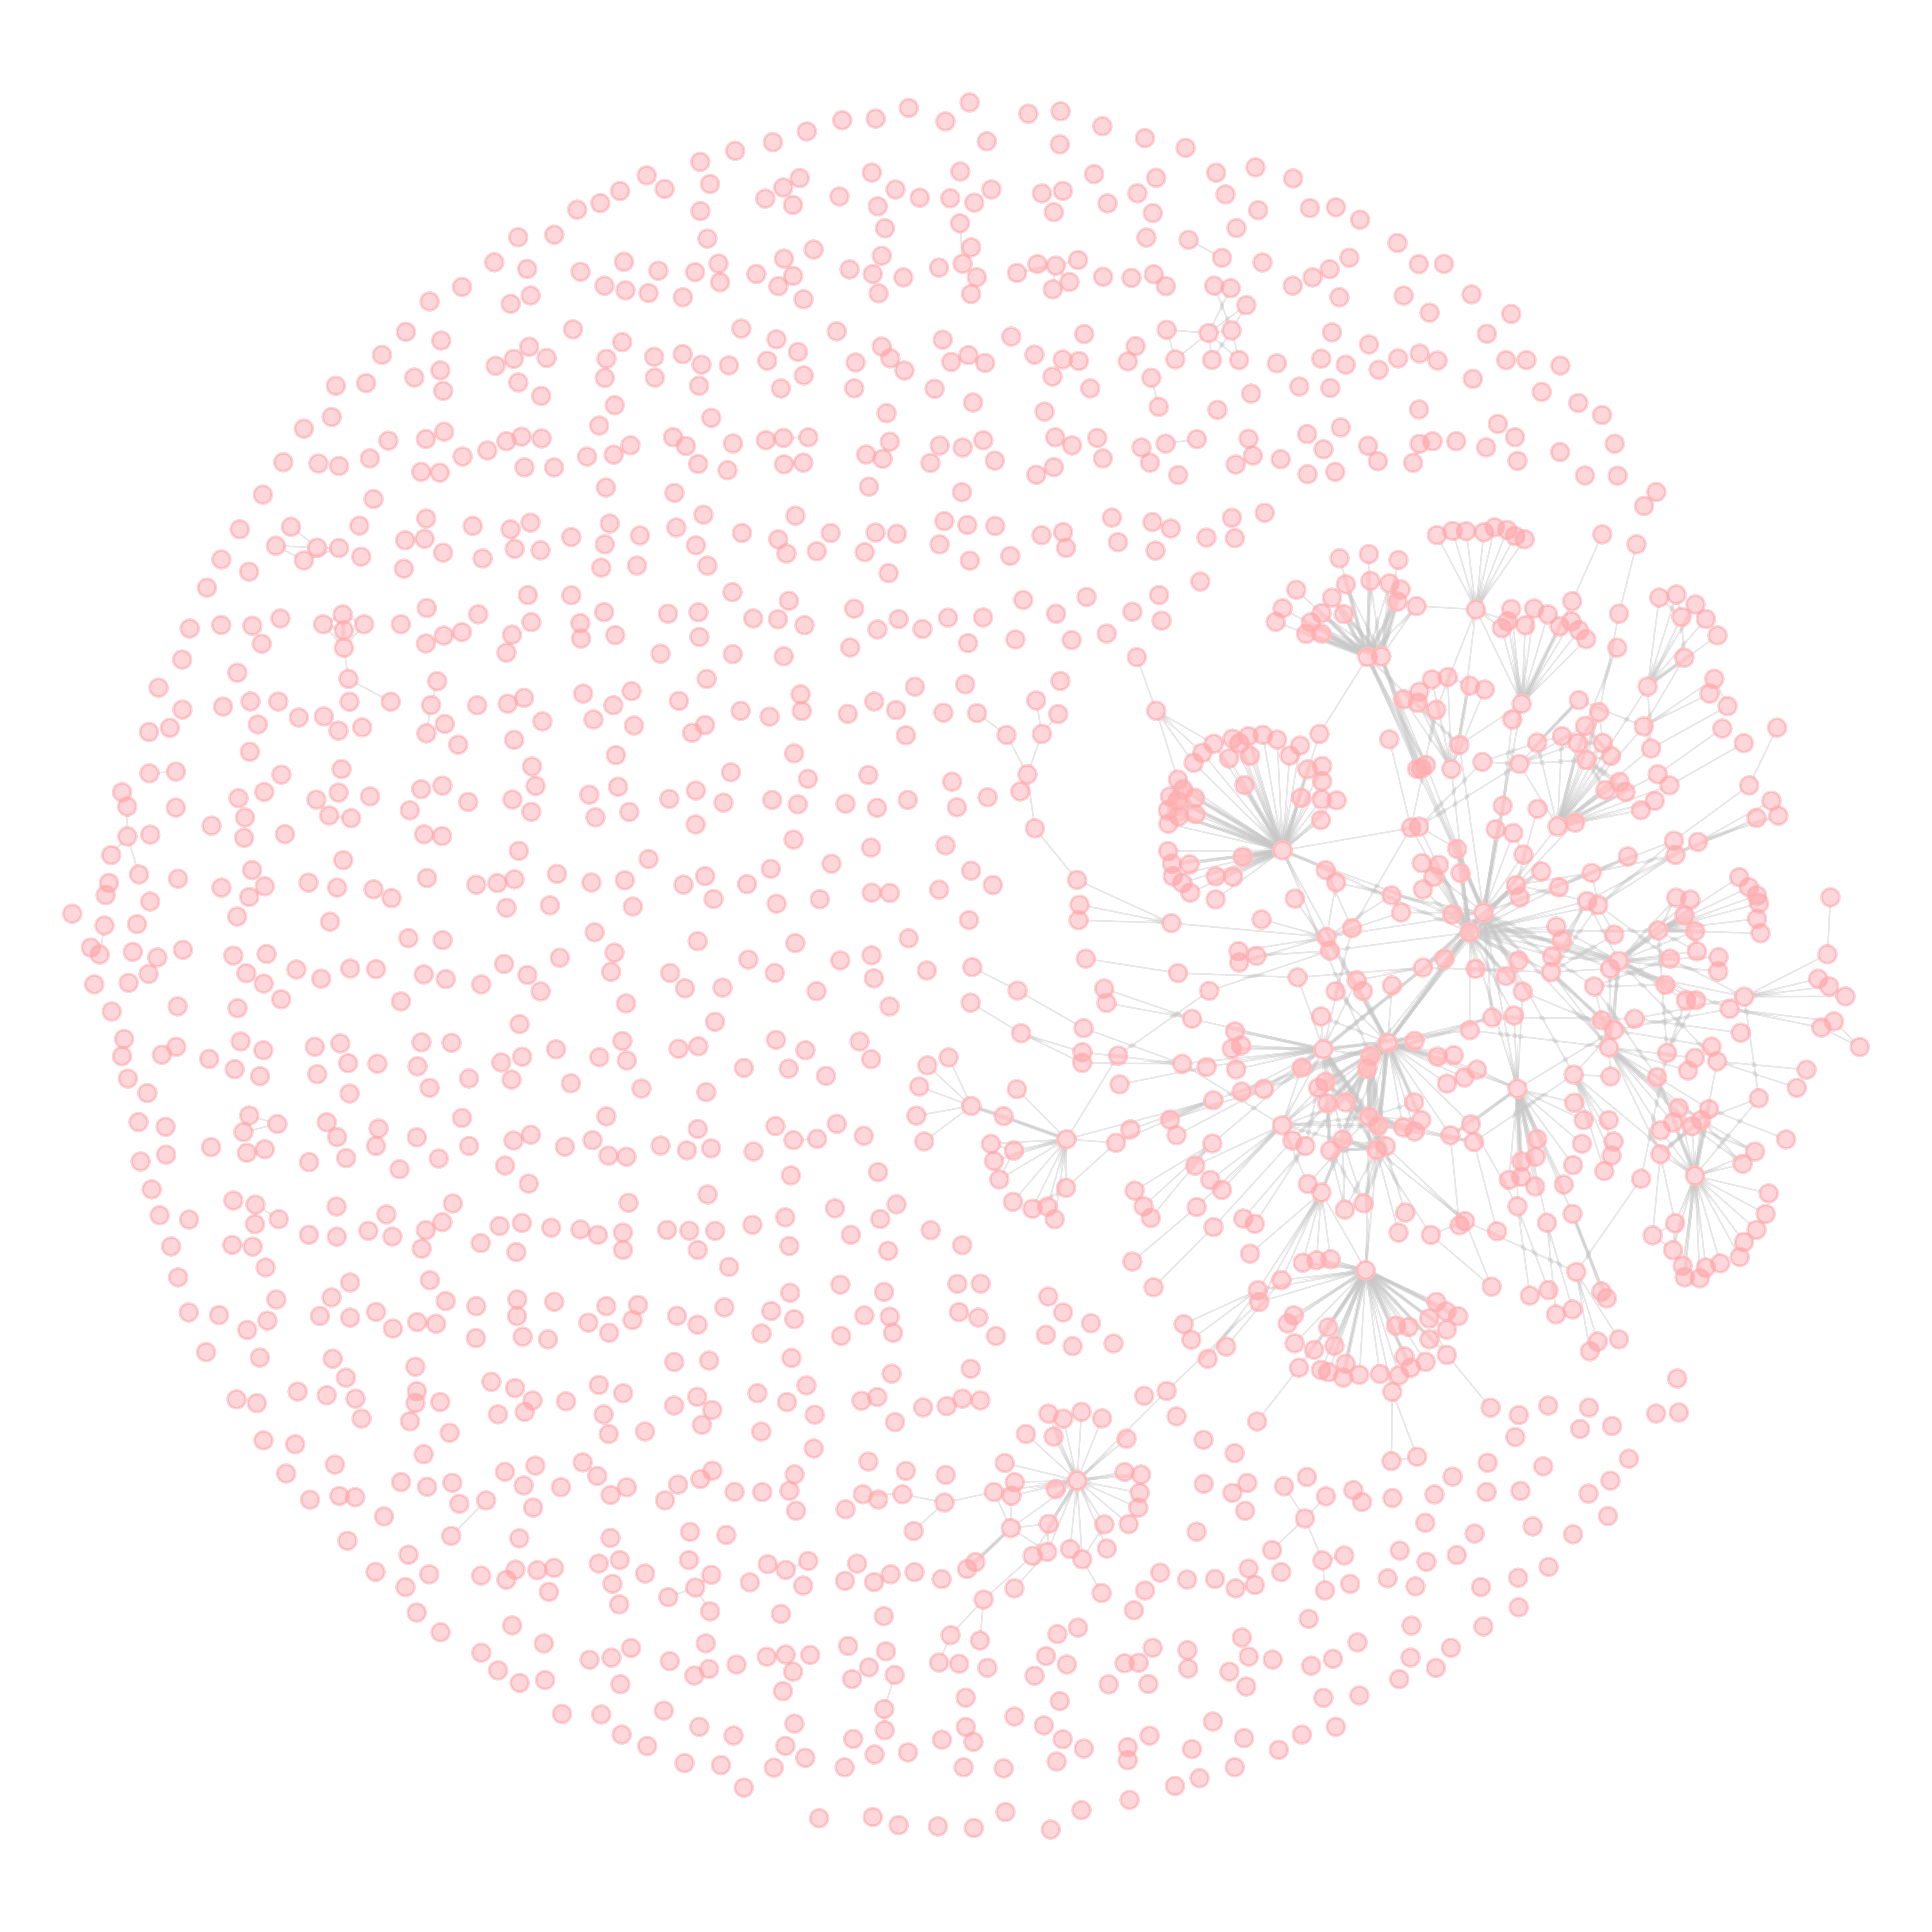
\includegraphics[width=\paperwidth]{graphics/katrinaplot.png}
\end{textblock*}

\begin{textblock*}{100mm}(20mm,0.3\textheight)
\begin{center}
\begin{itemize}
\item[\textbf{1)}] Overview of TERGM with \& w/o vertex dynamics
\begin{itemize}
\item Dynamic network logistic regression w/ \& w/o vertex dynamics
\end{itemize}
\item[\textbf{2)}] Bayesian TERGM 
\begin{itemize}
\item Bayesian analysis of DNR w/ \& w/o vertex dynamics
\end{itemize}
\item[\textbf{3)}] Empirical test cases
\begin{itemize}
\item DNC-RNC blog citation network
\item Lin Freeman's windsurfer network
\end{itemize}
\end{itemize}
\end{center}
\end{textblock*}

%----------- Fix name --------------------------------------------------%
\begin{textblock*}{100mm}(4mm,1.02\textheight)

\includegraphics[width=20mm,heighth=5mm ]{graphics/white.png}
\end{textblock*}

\begin{textblock*}{100mm}(4mm,1.02\textheight)
\emph{\tiny{\darkblue{Zack W Almquist, Sociology and Statistics, UMN}}}
\end{textblock*}
%----------- Fix name --------------------------------------------------%

\end{frame}



%----------- slide --------------------------------------------------%
\begin{frame}[t]{Road Map}

\begin{textblock*}{100mm}(20mm,0.3\textheight)
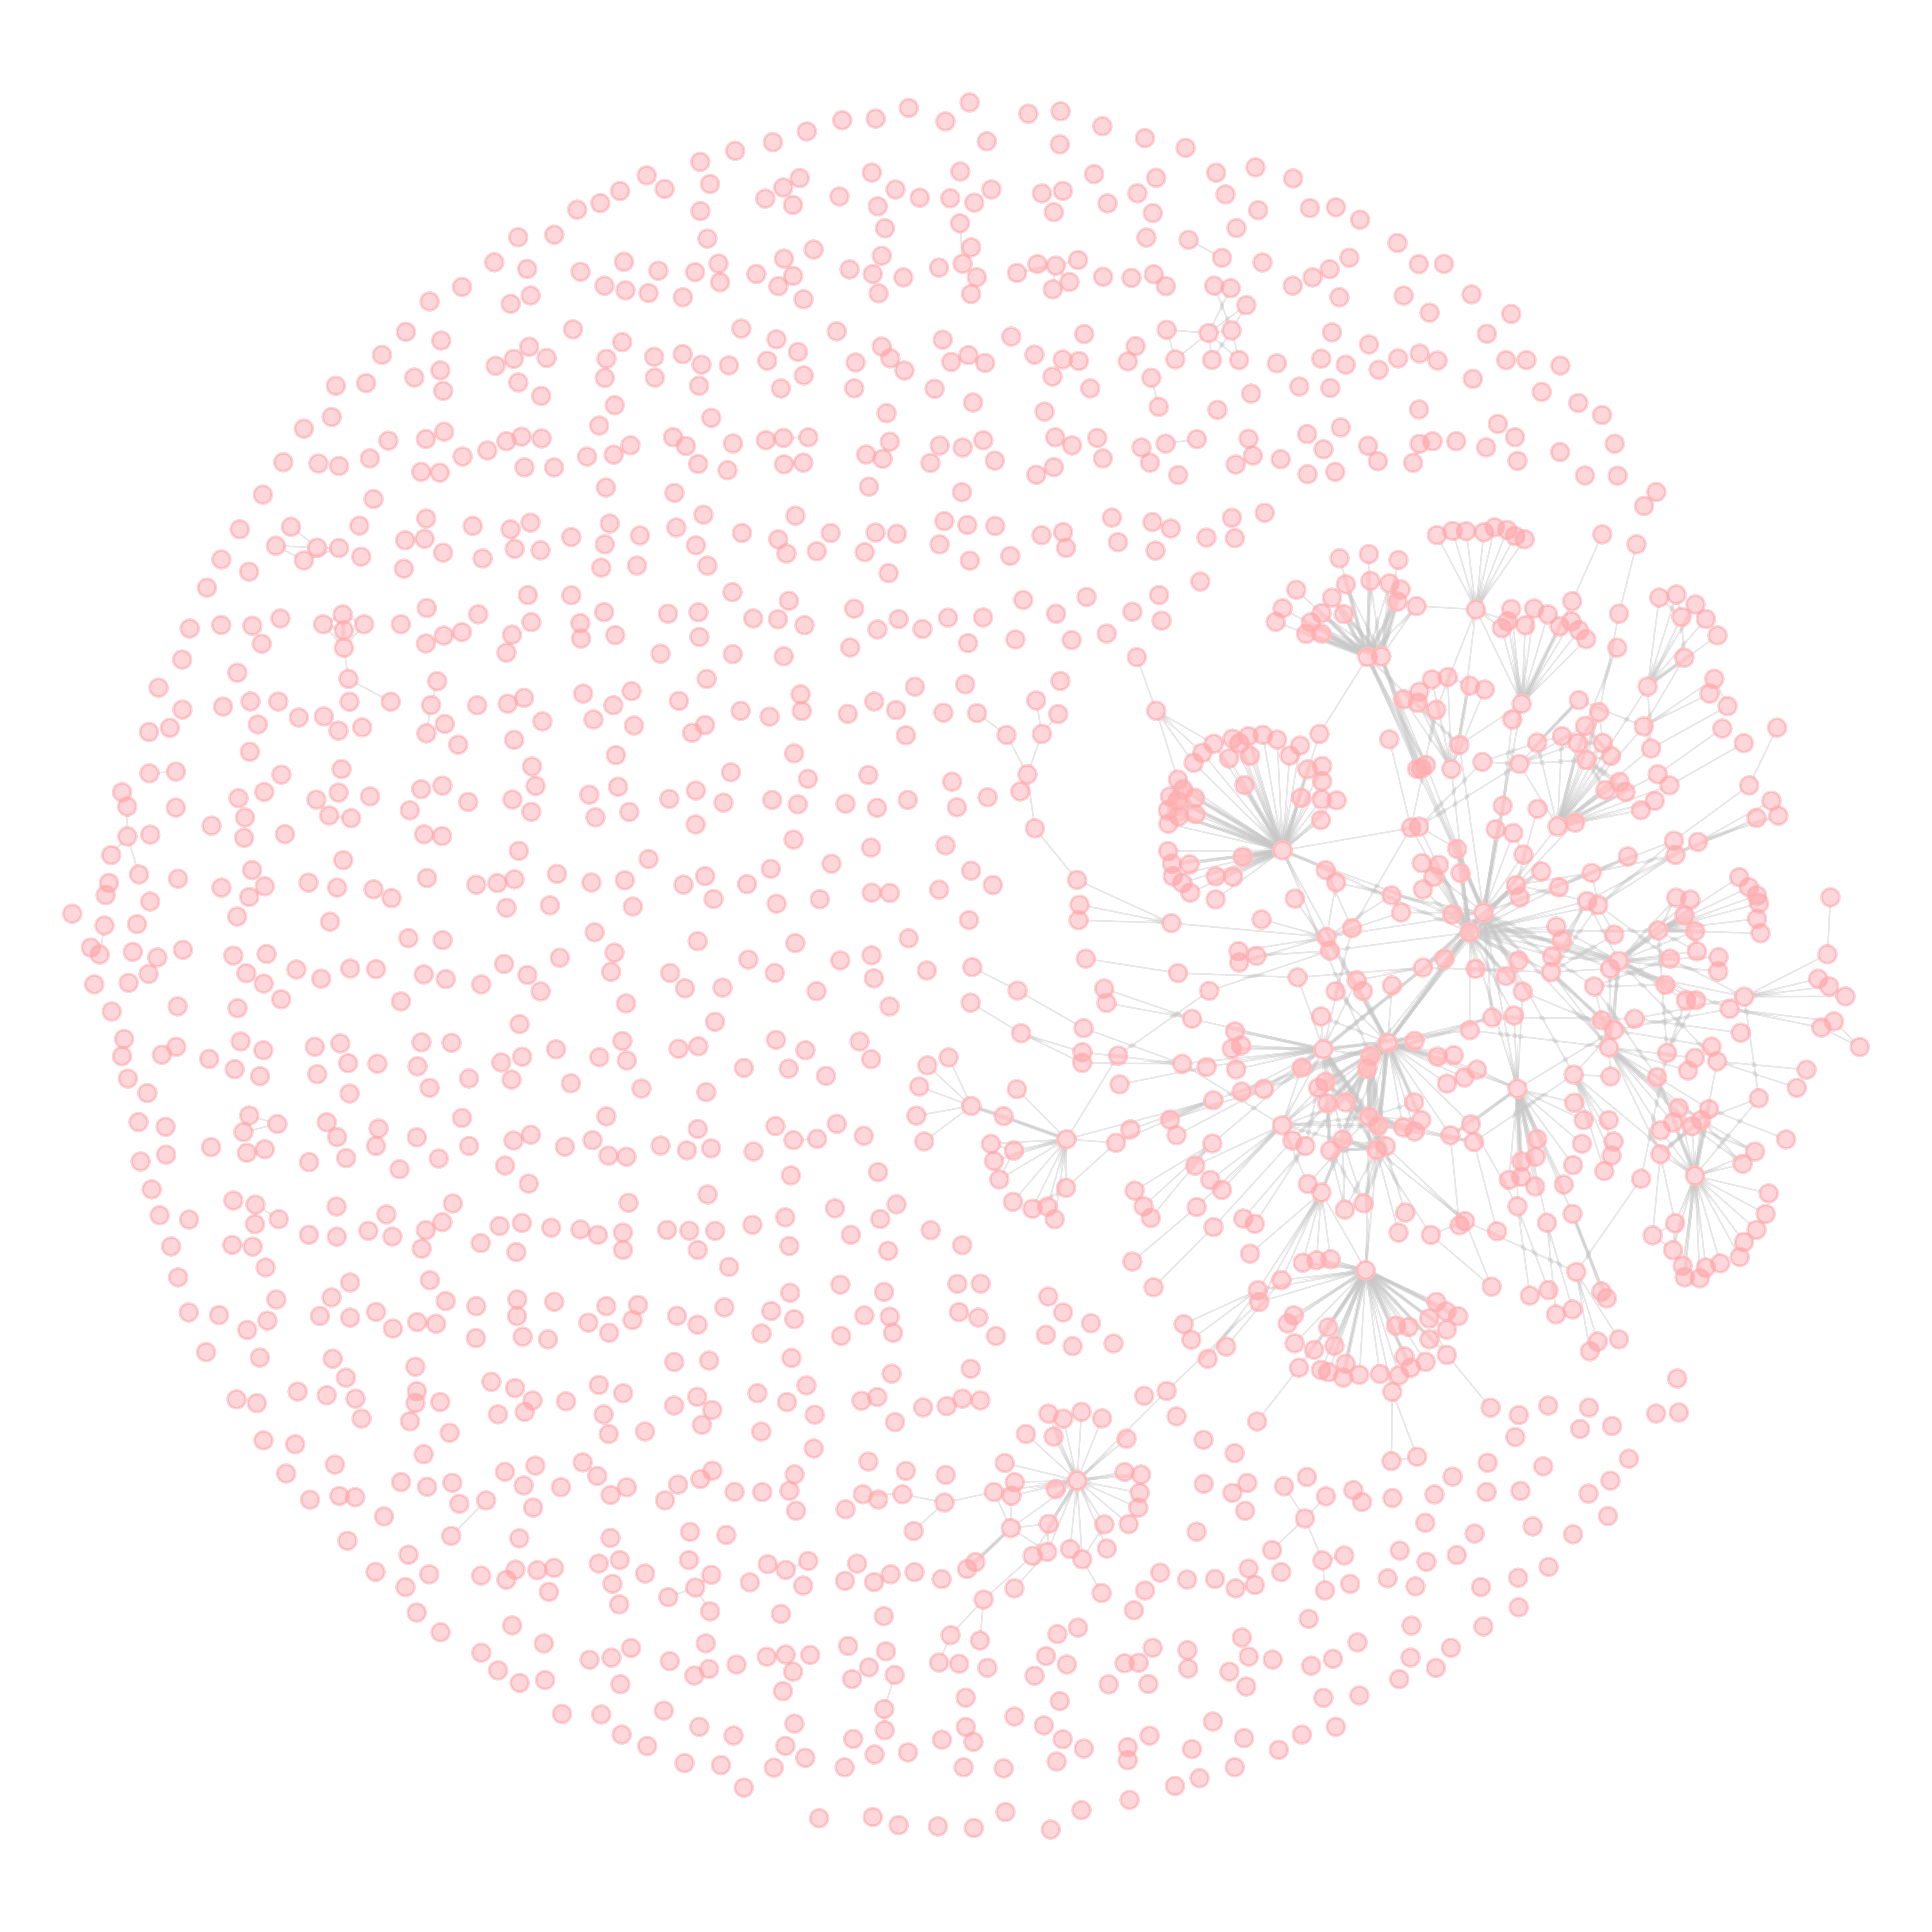
\includegraphics[width=\paperwidth]{graphics/katrinaplot.png}
\end{textblock*}

\begin{textblock*}{100mm}(20mm,0.3\textheight)
\begin{center}
\begin{itemize}
\item[\textcolor{light-gray}{\textbf{1)}}]\textcolor{light-gray}{Overview of TERGM with \& w/o vertex dynamics}
\begin{itemize}
\item[\textcolor{light-gray}{$\bullet$}] \textcolor{light-gray}{Dynamic network logistic regression w/ \& w/o vertex dynamics}
\end{itemize}
\item[\textbf{2)}] Bayesian TERGM 
\begin{itemize}
\item Bayesian analysis of DNR w/ \& w/o vertex dynamics
\end{itemize}
\item[\textbf{3)}] Empirical test cases
\begin{itemize}
\item DNC-RNC blog citation network
\item Lin Freeman's windsurfer network
\end{itemize}
\end{itemize}
\end{center}
\end{textblock*}

%----------- Fix name --------------------------------------------------%
\begin{textblock*}{100mm}(4mm,1.02\textheight)

\includegraphics[width=20mm,heighth=5mm ]{graphics/white.png}
\end{textblock*}

\begin{textblock*}{100mm}(4mm,1.02\textheight)
\emph{\tiny{\darkblue{Zack W Almquist, Sociology and Statistics, UMN}}}
\end{textblock*}
%----------- Fix name --------------------------------------------------%

\end{frame}

%----------- slide --------------------------------------------------%



%----------- reference ----------------------------------------------%
%\begin{frame}[allowframebreaks] 
%\addtocounter{framenumber}{-2}
%\addtocounter{framenumber}{-3}
%\frametitle{References}
%\def\newblock{}
%\bibliographystyle{ajs}
%\bibliography{bayesLogit}
%\end{frame}
%----------- reference ----------------------------------------------%






%%%%%%%%%%%%%%%
\begin{textblock*}{50mm}(70mm,.2\textheight)
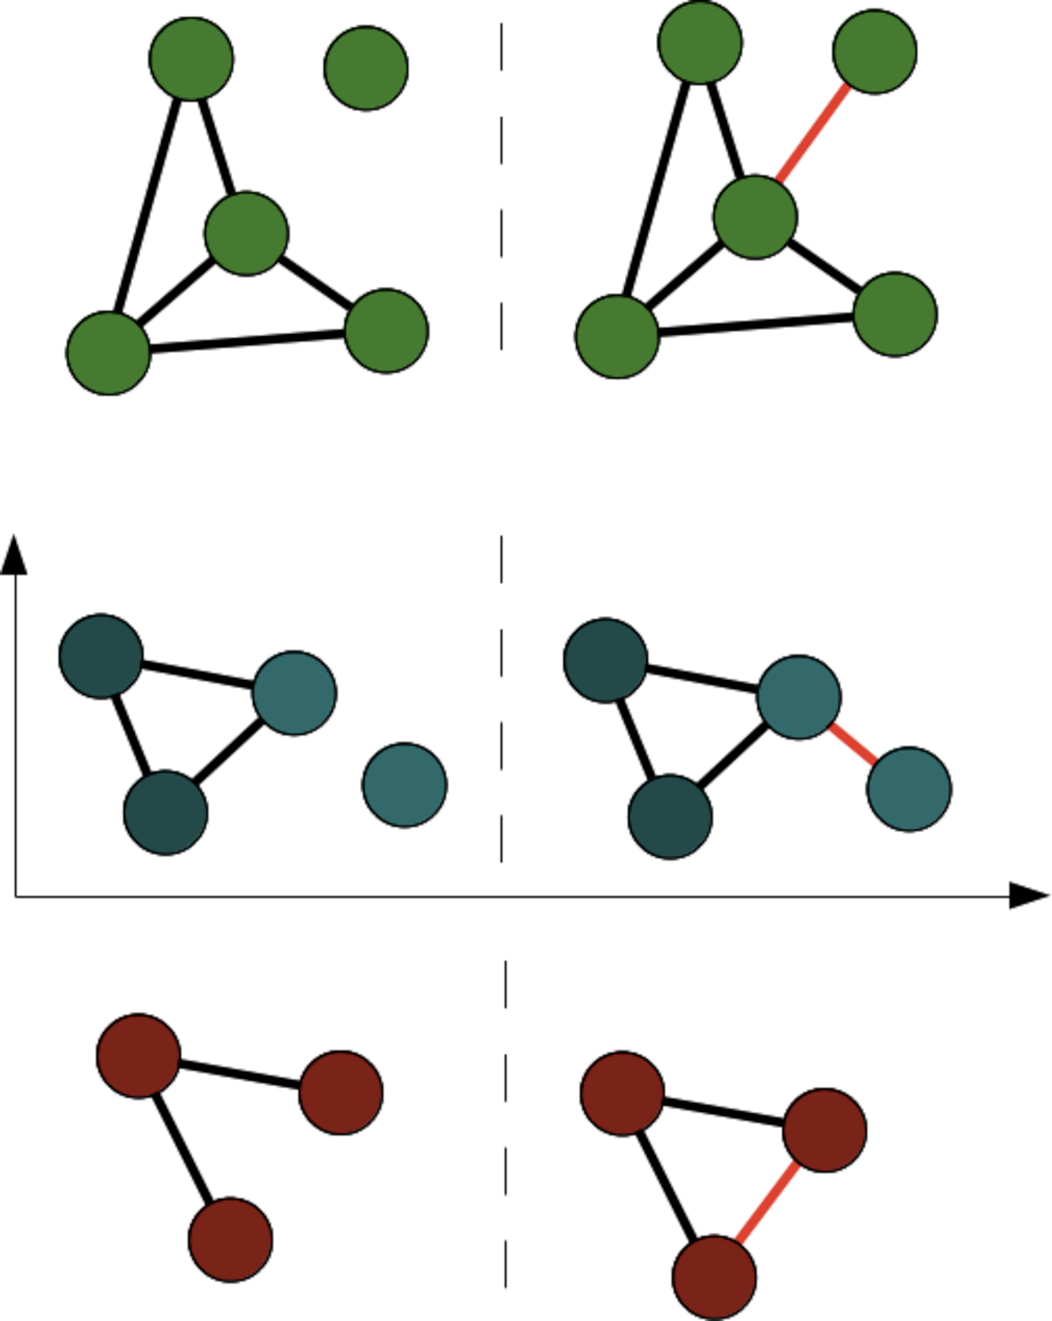
\includegraphics[width=1\linewidth]{graphics/exampleNetwork2.pdf} 
\end{textblock*}

\begin{textblock*}{60mm}(5mm,.25\textheight)
\begin{block}{Initial Intuition: Factors in Tie Formation over Time}
\begin{itemize}
\item All ties are not equally probable 
\begin{itemize}
\item Chance of an $(i,j)$ edge may depend on properties of $i$, $j$ and $t$
\item Can also depend on other $(i,j,t)$ relationships
\end{itemize}
\item Some examples:
\begin{itemize}
\item Homophily
\item Propinquity
\item Triadic/clustering effects
\begin{itemize}
\item Shared partner effects
\end{itemize}
\end{itemize}
\end{itemize}
\end{block}
\end{textblock*}
}
